\subsection{Menu}\label{menu}
Via een aparte sectie in de beheeromgeving kunnen de beschikbare menu's worden aangepast. Het menu systeem staat in Drupal los van de inhoud (nodes). 

In Drupal worden menu's en menu-items niet automatisch aangemaakt. Voor elk content-item moet je desgewenst een menu-item aanmaken. Een menu-item aanmaken kan dus pas nadat je het content-item hebt aangemaakt.

Ga naar \drupalpath{admin/structure/menu} om het overzicht van alle beschikbare menu's te bekijken. 

\bigskip

\begin{center}
	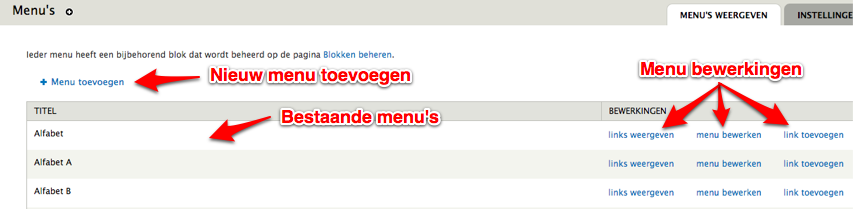
\includegraphics[width=\textwidth]{img/menu1.png}
\end{center}

\subsubsection{Menu-items bewerken}\label{menuitemsbewerken}
Alle menu-items kunnen bewerkt en verwijderd worden. Om een goed overzicht te krijgen van het menu dat je wil bewerken, klik je eerst op \emph{Links weergeven} bij het betreffende menu dat je wil bewerken. De onderstaande afbeelding toont waar alle opties staan.

\bigskip

\begin{center}
	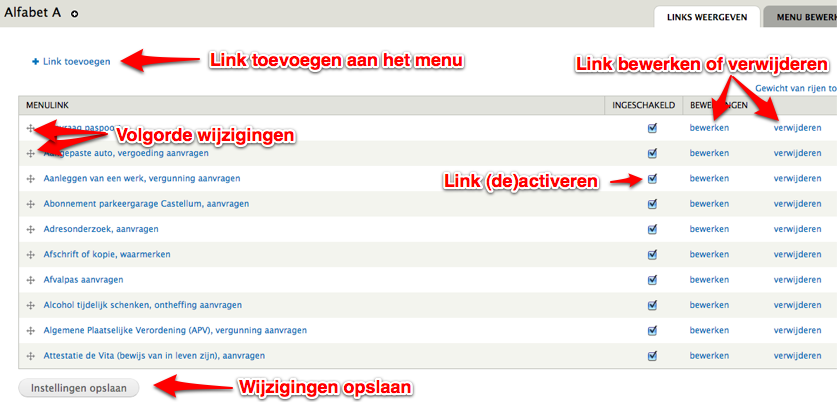
\includegraphics[width=\textwidth]{img/menu2.png}
\end{center}

Klik op \emph{bewerken} bij het betreffende menu-item om het menu-item te gaan bewerken. Na het bewerken klik je onderaan de pagina op de knop \emph{Opslaan} om de wijzigingen op te slaan.


\subsubsection{Menu-items toevoegen}\label{menuitemstoevoegen}

Om een goed overzicht te krijgen van het menu dat je wil bewerken, klik je eerst op \emph{Links weergeven} bij het betreffende menu waaraan je een menu-item wil toevoegen. Klik vervolgens op \emph{Link toevoegen}. 

Vul een titel in (dit wordt de klikbare tekst) en het pad waarnaar de link toe moet gaan. Als je een menu-item wil koppelen aan een node vul je bij het veld \emph{pad}, 'node/nodeID' in. Als je het menu-item wil koppelen aan een node met het ID \emph{123}, vul je 'node/123' in. 

Het is ook mogelijk een alias i.p.v. een node met een ID in te vullen. Node met het ID \emph{123} heeft bijvoorbeeld de alias \emph{pagina123}, vul dan bij het veld \emph{pad}, de alias \emph{pagina123} in. 

Klik vervolgens onderaan de pagina op de knop \emph{Opslaan}.

Herhaal deze stappen om meerdere menu-items toe te voegen.  

\subsubsection{Menu-items verwijderen}\label{menuitemsverwijderen}

Om een goed overzicht te krijgen van het menu dat je wil bewerken, klik je eerst op \emph{Links weergeven} bij het betreffende menu waarin je menu-items wil verwijderen. Klik op \emph{verwijderen} bij het betreffende menu-item om het menu-item te verwijderen. Na het bevestigen zal het menu-item permanent en onherstelbaar verwijderd worden.


\subsubsection{Alfabet}\label{alfabet}

\drupalpath gebruikt een \emph{Alfabet menu}. Dit menu(alfabet) bestaat uit een hoofdmenu met alle letters van het alfabet. Aan elke letter van het alfabet is een bijbehorend menu gekoppeld. Het menu voor de letter \emph{A} heet \emph{Alfabet A} en het menu voor de letter \emph{B} heet \emph{Alfabet B}. De werkwijze van het bewerken, toevoegen en verwijderen voor de alfabetische menu\emph{s is gelijk aan de werkwijze voor alle andere menu}s op \drupalpath{}.

\bigskip

Overzicht alfabet menu's

\begin{center}
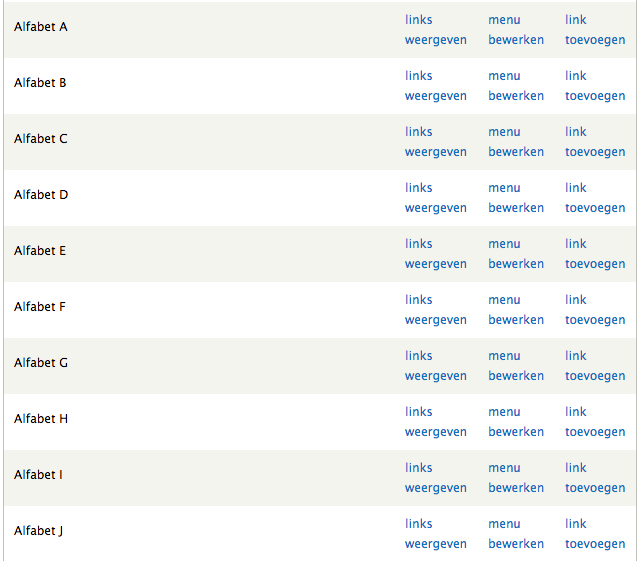
\includegraphics[width=0.5\textwidth]{img/menus_alfabet.png}
\end{center}

Overzicht alfabet menu A

\begin{center}
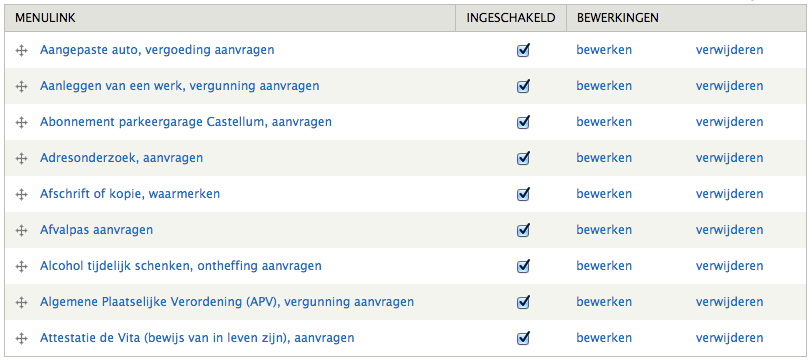
\includegraphics[width=\textwidth]{img/menu_alfabet_a.png}
\end{center}

\begin{center}

\includegraphics[width=\textwidth]{img/menu3.png}
\end{center}

\bigskip

\subsubsection{Main menu}\label{mainmenu}

\begin{center}
	
\includegraphics[width=\textwidth]{img/menu_main.png}
\end{center}

Menu locatie op \drupalpath{}: midden bovenaan de pagina. De werkwijze van het bewerken, toevoegen en verwijderen voor de alfabetische menu\emph{s is gelijk aan de werkwijze voor alle andere menu}s op \drupalpath{}. 

De verhouding tussen de verschillende niveau's en hun weergave op de website is te zien in de onderstaande afbeeldingen. Het 1ste niveau is te zien in de blauwe balk bovenaan op de website, het hoofdmenu (Figure 1). Het 2e niveau is te zien als dropdown/submenu onder het item in de blauwe balk en als hoofditem in het Submenublok. Het 3e niveau is te zien als submenu onder het 2e niveau in het Submenublok (Figure 2). Dieper dan drie niveau's wordt niet weergegeven in zowel het hoofdmenu als in het submenublok.

\begin{figure}[h!]
  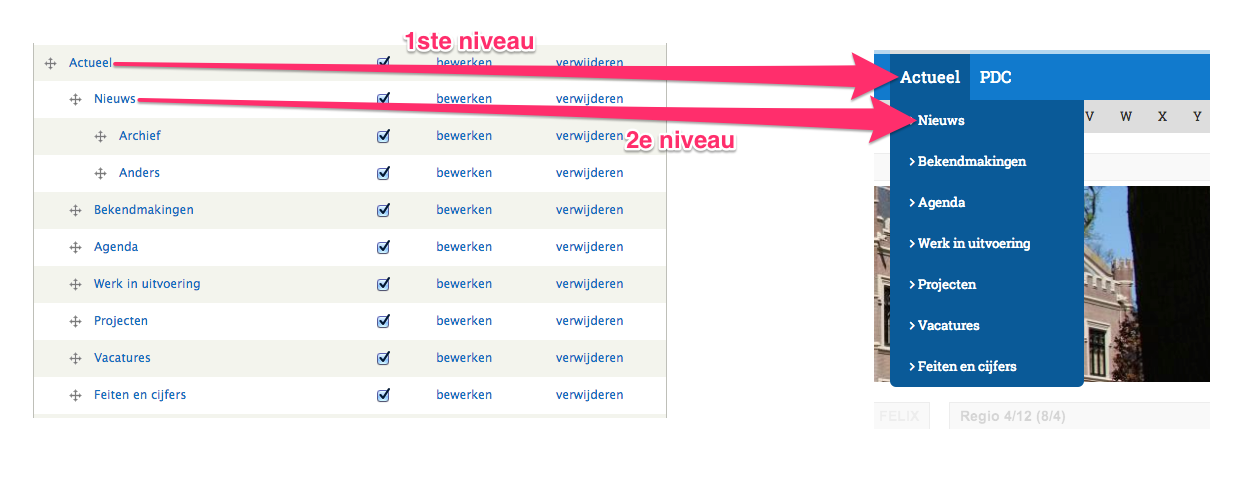
\includegraphics[width=\textwidth]{img/menu_mainmenu.png}
  \caption{Hoofdmenu}
\end{figure}

\begin{figure}[h!]
  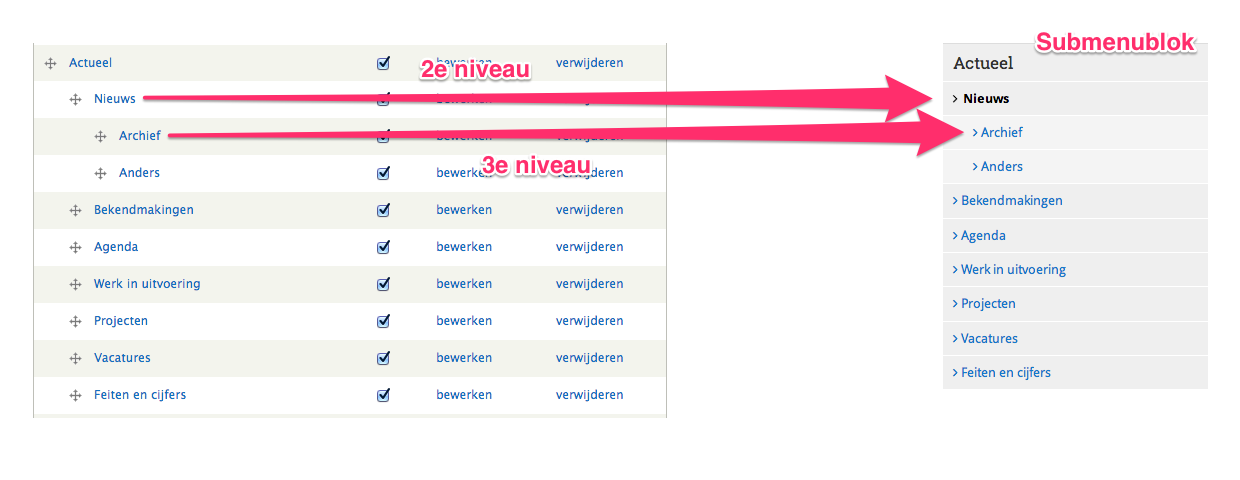
\includegraphics[width=\textwidth]{img/menu_submenu.png}
  \caption{Submenu}
\end{figure}

\bigskip

Vanwege de performance kunnen de menu's gecached worden. Dit zal er toe kunnen leiden dat wijzigingen niet direct zichtbaar zijn. De cache kan geleegd worden door een gebruiker met de juiste rechten of deze zal automatisch geleegd worden na verloop van tijd.

\bigskip

\subsubsection{Meta menu links}\label{metamenulinks}
Menu locatie op \drupalpath{}: links bovenaan de pagina. De werkwijze van het bewerken, toevoegen en verwijderen voor de alfabetische menu\emph{s is gelijk aan de werkwijze voor alle andere menu}s op \drupalpath{}. Dit menu kent geen subniveaus.
\bigskip

\begin{center}
	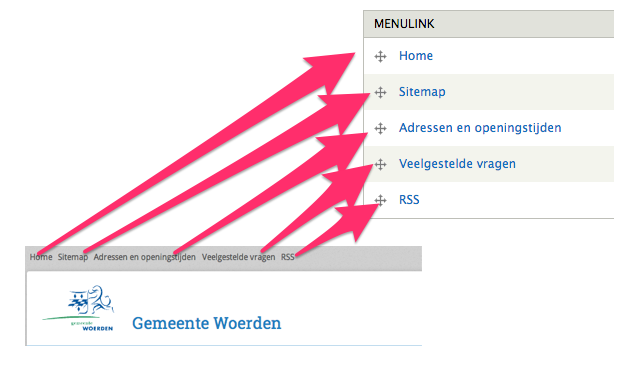
\includegraphics[width=\textwidth]{img/meta-menu.png}
\end{center}

\bigskip

\subsubsection{Meta menu rechts}\label{metamenurechts}
Menu locatie op \drupalpath{}: rechts bovenaan de pagina. De werkwijze van het bewerken, toevoegen en verwijderen voor de alfabetische menu\emph{s is gelijk aan de werkwijze voor alle andere menu}s op \drupalpath{}. Dit menu kent geen subniveaus.
\bigskip

\begin{center}
	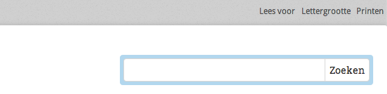
\includegraphics[width=\textwidth]{img/menu_metarechts.png}
\end{center}

\bigskip

\subsubsection{Toptaken}\label{toptaken}
Menu locatie op \drupalpath{}: links midden op de voorpagina. De werkwijze van het bewerken, toevoegen en verwijderen voor de alfabetische menu\emph{s is gelijk aan de werkwijze voor alle andere menu}s op \drupalpath{}. Voor het beste resultaat is aan te houden om maximaal 5 hoofdniveaus en maximaal 6 subniveaus, per hoofdniveau, aan te maken.

\bigskip

\begin{center}
	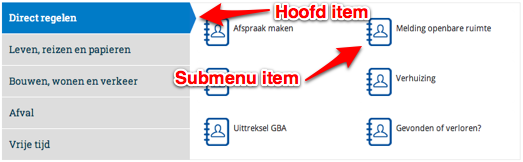
\includegraphics[width=\textwidth]{img/menu_toptaken.png}
\end{center}

\begin{center}
	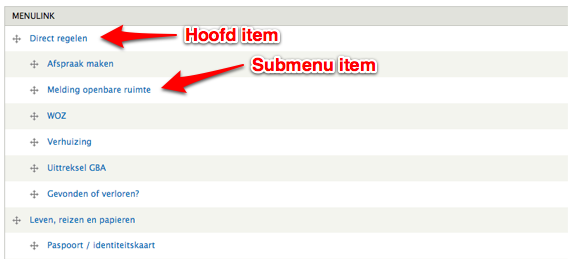
\includegraphics[width=\textwidth]{img/menu_toptaken2.png}
\end{center}